\documentclass[11pt]{article}

\usepackage[a4paper,margin=1in]{geometry}
\usepackage[T1]{fontenc}
\usepackage[utf8]{inputenc}
\usepackage{lmodern}
\usepackage{microtype}
\usepackage{amsmath,amssymb,amsthm,mathtools,mathrsfs}
\usepackage{booktabs,array}
\usepackage{graphicx}
\usepackage{float}
\usepackage[section]{placeins}
\usepackage{enumitem}
\usepackage[numbers,sort&compress]{natbib}
\usepackage{xcolor}
\usepackage{xurl}
\usepackage[colorlinks=true,linkcolor=blue!55!black,citecolor=blue!55!black,urlcolor=blue!55!black]{hyperref}
\usepackage[nameinlink,noabbrev]{cleveref}

\setlength{\parindent}{1.4em}
\setlength{\parskip}{0.12em}
\setlist{itemsep=0.25em,topsep=0.35em}

\newtheorem{theorem}{Theorem}[section]
\newtheorem{proposition}[theorem]{Proposition}
\newtheorem{lemma}[theorem]{Lemma}
\newtheorem{corollary}[theorem]{Corollary}
\theoremstyle{definition}
\newtheorem{definition}[theorem]{Definition}
\newtheorem{condition}[theorem]{Condition}
\theoremstyle{remark}
\newtheorem{remark}[theorem]{Remark}

\newcommand{\R}{\mathbb R}
\newcommand{\C}{\mathbb C}
\newcommand{\Id}{\mathrm I}
\newcommand{\cK}{\mathcal K}
\newcommand{\cB}{\mathcal B}
\newcommand{\cQ}{\mathcal Q}
\newcommand{\cD}{\mathcal D}
\newcommand{\cF}{\mathcal F}
\newcommand{\cG}{\mathcal G}
\newcommand{\cH}{\mathcal H}
\newcommand{\uc}{u_{\mathrm c}}
\newcommand{\norm}[1]{\left\lVert #1\right\rVert}
\newcommand{\tr}{\operatorname{tr}}
\newcommand{\detF}{\operatorname{det}}
\newcommand{\Dettwo}{\operatorname{det}\nolimits_2}

\title{Small-Noise Mesh Laws and the Double-Pole Obstruction\\
\large for Intrinsic Bulk Two-Step Fredholm Determinants}
\author{Liang Wang}
\date{July 2026}

\begin{document}
\maketitle

\begin{abstract}
At every fixed positive noise width, the Perron/parity-deflated
folded-Gaussian operator has an intrinsic trace-class square and a strict
Fredholm determinant.  The next problem contains two logically independent
limits: spatial resolution $n\to\infty$ and noise width
$\sigma\downarrow0$.  We separate them.

First, for $0<\sigma\le0.03$, explicit Gaussian-moment estimates give
\[
 \norm{\cK_\sigma}_{\mathfrak S_2}
 \le A_0\sigma^{-1/2},
 \qquad
 \norm{(k_\sigma)_x}_{L^2}
 +\norm{(k_\sigma)_y}_{L^2}
 \le A_1\sigma^{-3/2},
\]
with
$A_0=2.124503864054395$ and
$A_1=11.373709849581182$.  If $G_{n,\sigma}$ is the orthogonal
cell-average Galerkin lift, then
\[
 \norm{G_{n,\sigma}-\cK_\sigma}_{\mathfrak S_2}
 \le\frac{A_1}{\pi n\sigma^{3/2}},
\]
and
\[
 \norm{G_{n,\sigma}^2-\cK_\sigma^2}_{\mathfrak S_1}
 \le
 \frac{15.38295583703884}{n\sigma^2}
 +\frac{13.10703757570889}{n^2\sigma^3}.
\]
Thus $n\sigma^{3/2}\to\infty$ is sufficient for one-step
Hilbert--Schmidt convergence, while $n\sigma^2\to\infty$ is sufficient for
two-step trace-norm convergence.  A normalized Gaussian row model proves
that the exponent $h\sigma^{-3/2}$ is sharp for cell projection, with exact
constant $(\sqrt{48}\,\pi^{1/4})^{-1}$.  On shrinking determinant disks
$|w|\le\rho\sigma$, the standard continuity estimate only requires
$n\sigma\to\infty$; on a fixed disk it develops an exponential
$e^{C_R/\sigma}$ wall.

Second, arbitrarily fine spatial resolution cannot produce a naive entire
small-noise limit.  The deterministic parity-centered one-step germ is
known exactly in the form
\[
 \widehat D_{0,\mathrm{bulk},2}(z)
 =\frac{\cG(z)}{1-z^2/\lambda},
 \qquad \lambda=1.678573510428322\ldots,
\]
where $\cG$ is holomorphic and nonzero for $|z|<\lambda$.  Symmetric
regularization therefore gives the two-step germ
\[
 \widehat\cF_0(w)
 =\frac{\cH(w)}{(1-w/\lambda)^2},
\]
where $\cH$ is holomorphic and nonzero for $|w|<\lambda^2$.  Hence
$w=\lambda$ is a genuine double pole.  Although every positive-noise
two-step determinant is entire and its Taylor coefficients converge, the
family is not locally bounded on any disk of radius greater than $\lambda$.

The canonical finite resolution of the pole is
\[
 S_N(w)=\Pi_N(w/\lambda)^2,
 \qquad \Pi_N(q)=1+q+\cdots+q^N,
\]
and its edge profile is
\[
 \frac{S_N(\lambda e^{s/(N+1)})}{(N+1)^2}
 \longrightarrow\left(\frac{e^s-1}{s}\right)^2.
\]
Archived resonance clouds exhibit this squared profile numerically.  The
remaining open gate is a uniform small-noise weighted-Riesz transport
theorem; it is stated explicitly rather than assumed silently.  No
arithmetic trace formula, self-adjoint Hilbert--P\'olya operator, or
Riemann-hypothesis claim is made.
\end{abstract}

\noindent\textbf{Keywords:} small noise; Hilbert--Schmidt approximation;
trace norm; Fredholm determinant; normal family; resonance cloud; Gaussian
kernel.

\medskip
\noindent\textbf{MSC 2020:} 47B10; 47A10; 65R20; 37M25; 30D45.

\section{Introduction}
\label{sec:introduction}

The fixed-noise spectral construction has reached a strict determinant.
For the folded-Gaussian Markov operator $\cK_\sigma$, the Perron and negative
parity weighted Riesz terms can be removed intrinsically at
$\sigma=10^{-2}$, giving
\[
 \cB_\sigma=\cK_\sigma-\cQ_{+,\sigma}-\cQ_{-,\sigma}.
\]
The preceding trace-ideal completion proved that full and adaptive
discretizations converge to $\cB_{10^{-2}}$ in Hilbert--Schmidt norm, their
squares converge in trace norm, and
\begin{equation}
 \detF(\Id-wB_{n,10^{-2}}^2)
 \longrightarrow
 \detF(\Id-w\cB_{10^{-2}}^2)
 \label{eq:fixed-noise-recalled}
\end{equation}
locally uniformly in $w$ \citep{WangTraceIdeal2026}.

It is tempting to let $\sigma$ decrease and merely increase the matrix
dimension.  This conflates two different obstructions.
\begin{enumerate}[leftmargin=2em]
 \item The Gaussian kernel becomes narrower and larger in
 Hilbert--Schmidt norm.  A grid schedule adequate for eigenvalue pictures
 need not make the lifted kernel converge in an absolute trace ideal.
 \item Even at infinite spatial resolution, the deterministic
 parity-centered target is meromorphic, not entire.  No mesh schedule can
 remove a genuine pole in the small-noise coefficient germ.
\end{enumerate}

The purpose of this paper is to separate those effects quantitatively.  The
first half derives an unconditional mesh law for the raw folded Gaussian
operator.  Its one-step scale is $n\sigma^{3/2}$, not the commonly used
$n\sigma$.  Squaring introduces the growing Hilbert--Schmidt size
$\norm{\cK_\sigma}_2=O(\sigma^{-1/2})$ and moves the sufficient trace-norm
scale to $n\sigma^2$.

The second half combines the fixed-noise symmetric determinant identity
with the exact deterministic pole theorem of the parity-extracted bulk
analysis \citep{WangBulkScattering2026}.  The simple poles at
$z=\pm\sqrt\lambda$ merge under $w=z^2$ into a double pole at
$w=\lambda$.  This gives a stronger conclusion than ``the numerical limit
looks unstable'': the family cannot be locally bounded on any disk crossing
that point.

The correct finite model is also forced.  A simple one-step pole is resolved
by the geometric polynomial $\Pi_N(z^2/\lambda)$.  The two-step symmetric
product squares this factor.  The resonance cloud therefore produces double
zeros in the $w$-plane and the universal edge profile is the square of the
one-step scattering profile.

\subsection*{Logical layers}

Four levels are kept distinct throughout.
\begin{description}[leftmargin=3.4cm,style=nextline]
 \item[Unconditional analytic theorem]
 Uniform Gaussian Hilbert--Schmidt bounds, cell-average Galerkin mesh laws,
 the sharp normalized-row exponent, the deterministic double pole, the
 normal-family obstruction, and the exact geometric square model.
 \item[Fixed-noise validated input]
 The $\sigma=10^{-2}$ intrinsic weighted-Riesz terms and strict bulk-square
 determinant from RH-45.
 \item[Conditional bulk route]
 A uniform small-noise bound for the peripheral weighted terms and their
 discretizations.  This is isolated as a named condition.
 \item[Floating diagnostic]
 Reprocessing of the archived RH-15 resonance clouds in the two-step
 variable.  It supports the geometric mechanism but proves no uniform
 contour theorem.
\end{description}

\section{Folded Gaussian family and cell lifts}
\label{sec:operator}

Let $\uc$ be the root in $(1.5,1.6)$ of
\begin{equation}
 u^3-2u^2+2u-2=0,
 \label{eq:critical-polynomial}
\end{equation}
and put $m(x)=1-\uc x^2$ for $x\in[0,1]$.  For $0<\sigma\le0.03$, define
\begin{align}
 g_\sigma(x,y)
 &=e^{-(y-m(x))^2/(2\sigma^2)}
  +e^{-(y+m(x))^2/(2\sigma^2)},
 \label{eq:raw-kernel}\\
 Z_\sigma(x)&=\int_0^1g_\sigma(x,y)\,dy,
 \qquad
 k_\sigma(x,y)=\frac{g_\sigma(x,y)}{Z_\sigma(x)},
 \label{eq:normalized-kernel}\\
 (\cK_\sigma f)(x)&=\int_0^1k_\sigma(x,y)f(y)\,dy.
 \label{eq:operator}
\end{align}
The omitted factor $(\sqrt{2\pi}\sigma)^{-1}$ cancels in the row
normalization.

Let $V_n$ be the space of functions constant on the cells
$I_{n,j}=[j/n,(j+1)/n)$, and let $E_n$ be the orthogonal projection onto
$V_n$.  The canonical cell-average Galerkin operator is
\begin{equation}
 G_{n,\sigma}=E_n\cK_\sigma E_n,
 \label{eq:galerkin}
\end{equation}
extended by zero on $V_n^\perp$.  The Euclidean matrix in the normalized
cell basis is isometric to this lift, so matrix Frobenius norm equals
operator Hilbert--Schmidt norm.

The distinction between \eqref{eq:galerkin} and a midpoint matrix matters
only for constants.  Cell averaging makes the leading small-noise exponent
transparent and gives an exact orthogonal projection.  Midpoint sampling,
row normalization, and adaptive cutoff are discussed after the leading law
has been established.

\section{Uniform Gaussian Hilbert--Schmidt envelope}
\label{sec:envelope}

The folded normalizer has a useful exact interpretation.  With $t=-y$ in
the second term of \eqref{eq:raw-kernel},
\begin{equation}
 Z_\sigma(x)
 =\int_{-1}^{1}
 e^{-(t-m(x))^2/(2\sigma^2)}\,dt.
 \label{eq:normalizer-unfolded}
\end{equation}
Since $m(x)\in[1-\uc,1]$ and $|1-\uc|<1$, the minimum occurs at
$m=1$.  Therefore
\begin{equation}
 Z_\sigma(x)
 \ge c_0\sigma,
 \qquad
 c_0=\sqrt{\frac\pi2}
 \operatorname{erf}\!\left(\frac{\sqrt2}{0.03}\right)
 =1.2533141373155\ldots.
 \label{eq:normalizer-lower}
\end{equation}

\begin{lemma}[Raw Gaussian row bounds]
\label{lem:raw-bounds}
Uniformly in $x$ and $0<\sigma\le0.03$,
\begin{align}
 \norm{g_\sigma(x,\cdot)}_{L^2(0,1)}
 &\le2\pi^{1/4}\sigma^{1/2},
 \label{eq:raw-L2}\\
 \norm{(g_\sigma)_y(x,\cdot)}_{L^2(0,1)}
 &\le\sqrt2\,\pi^{1/4}\sigma^{-1/2},
 \label{eq:raw-y}\\
 \norm{(g_\sigma)_m(x,\cdot)}_{L^2(0,1)}
 &\le\sqrt2\,\pi^{1/4}\sigma^{-1/2},
 \label{eq:raw-m}\\
 |(Z_\sigma)_m(x)|&\le1.
 \label{eq:Z-m}
\end{align}
\end{lemma}

\begin{proof}
Use $(a+b)^2\le2(a^2+b^2)$ and enlarge each target integral to the real
line.  The required moments are
\[
 \int_\R e^{-t^2/\sigma^2}\,dt=\sqrt\pi\sigma,
 \qquad
 \int_\R\frac{t^2}{\sigma^4}e^{-t^2/\sigma^2}\,dt
 =\frac{\sqrt\pi}{2\sigma}.
\]
Differentiating \eqref{eq:normalizer-unfolded} in the center gives a
difference of two endpoint exponentials, both in $[0,1]$, proving
\eqref{eq:Z-m}.
\end{proof}

\begin{theorem}[Explicit small-noise envelope]
\label{thm:envelope}
For $0<\sigma\le0.03$,
\begin{align}
 \norm{\cK_\sigma}_{\mathfrak S_2}
 &\le A_0\sigma^{-1/2},
 \qquad
 A_0=\frac{2\pi^{1/4}}{c_0}
 \le2.124503864054395,
 \label{eq:kernel-envelope}\\
 \norm{(k_\sigma)_x}_{L^2([0,1]^2)}
 +\norm{(k_\sigma)_y}_{L^2([0,1]^2)}
 &\le A_1\sigma^{-3/2},
 \qquad
 A_1\le11.373709849581182.
 \label{eq:first-envelope}
\end{align}
\end{theorem}

\begin{proof}
Equation \eqref{eq:kernel-envelope} follows from
\eqref{eq:normalizer-lower} and \eqref{eq:raw-L2}.  The target derivative follows from
\eqref{eq:raw-y}.  For the center derivative,
\begin{equation}
 (k_\sigma)_m
 =\frac{(g_\sigma)_m}{Z_\sigma}
 -\frac{g_\sigma(Z_\sigma)_m}{Z_\sigma^2},
 \label{eq:center-quotient}
\end{equation}
so \cref{lem:raw-bounds} gives
\begin{equation}
 \norm{(k_\sigma)_m(x,\cdot)}_2
 \le\pi^{1/4}
 \left(\frac{\sqrt2}{c_0}+\frac2{c_0^2}\right)
 \sigma^{-3/2}.
 \label{eq:center-bound}
\end{equation}
Finally, $|m'(x)|\le2\uc$.  Adding the source and target constants yields
$A_1$.
\end{proof}

The estimates are deliberately coarse.  At $\sigma=10^{-2}$ they give
\[
 \norm{\cK_\sigma}_2\le21.2451,
 \qquad
 \norm{k_x}_2+\norm{k_y}_2\le11373.8,
\]
whereas the 160-bit fixed-noise certificate gives $5.49855$ and
$1052.04$.  The present constants are larger because they remain valid
uniformly down to zero noise without interval integration at every width.

\section{The sharp Gaussian-row projection exponent}
\label{sec:sharp-row}

The power $\sigma^{-3/2}$ is not merely an artifact of the upper bound.
Consider the normalized Gaussian density on $\R$,
\begin{equation}
 f_\sigma(y)=\frac1{\sqrt{2\pi}\sigma}
 e^{-y^2/(2\sigma^2)},
 \label{eq:gaussian-row}
\end{equation}
and let $P_h$ denote orthogonal averaging on cells of width $h$.

\begin{theorem}[Sharp cell-average row law]
\label{thm:sharp-row}
As $h/\sigma\to0$,
\begin{equation}
 \norm{f_\sigma-P_hf_\sigma}_{L^2(\R)}
 \sim C_{\mathrm G}h\sigma^{-3/2},
 \qquad
 C_{\mathrm G}
 =\frac1{\sqrt{48}\,\pi^{1/4}}
 =0.1084156338230097\ldots.
 \label{eq:sharp-row-law}
\end{equation}
The law is independent of the phase of the cell grid relative to the
Gaussian center.
\end{theorem}

\begin{proof}
The standard cell-average expansion gives
\begin{equation}
 \norm{f-P_hf}_2^2
 =\frac{h^2}{12}\norm{f'}_2^2+o(h^2)
 \label{eq:cell-average-expansion}
\end{equation}
for $f\in H^1(\R)$; translation of the grid changes only the lower-order
term.  Direct Gaussian integration gives
\[
 \norm{f_\sigma'}_2^2
 =\frac1{4\sqrt\pi\sigma^3}.
\]
Insert this in \eqref{eq:cell-average-expansion}.
\end{proof}

There is also an exact scaling identity.  If $a=h/\sigma$, then
\begin{equation}
 \norm{f_\sigma-P_hf_\sigma}_2
 =\sigma^{-1/2}E(a),
 \qquad
 E(a)\sim C_{\mathrm G}a.
 \label{eq:row-scaling}
\end{equation}
The numerical pilot evaluates every projected cell mass by differences of
the normal distribution function.  At $a=2^{-9}$, the scaled constant is
within $9.49\times10^{-8}$ relative error of $C_{\mathrm G}$.

The row theorem does not by itself give a lower bound for the complete
folded operator, because source averaging and boundary conditioning add
geometry.  It does show that the exponent in \eqref{eq:first-envelope} is
the natural absolute-$L^2$ cell-resolution exponent for a Gaussian row.

\section{One-step and two-step mesh laws}
\label{sec:mesh-laws}

The tensor Poincar\'e--Wirtinger inequality and
\cref{thm:envelope} immediately give the leading grid law.

\begin{theorem}[Explicit cell-average mesh bounds]
\label{thm:mesh-bounds}
For every $n\ge2$ and $0<\sigma\le0.03$,
\begin{equation}
 \varepsilon_{n,\sigma}
 :=\norm{G_{n,\sigma}-\cK_\sigma}_{\mathfrak S_2}
 \le\frac{A_1}{\pi n\sigma^{3/2}}
 \le\frac{3.620364287707642}{n\sigma^{3/2}}.
 \label{eq:hs-mesh-bound}
\end{equation}
Moreover,
\begin{align}
 \delta_{n,\sigma}
 &:=\norm{G_{n,\sigma}^2-\cK_\sigma^2}_{\mathfrak S_1}
 \notag\\
 &\le\varepsilon_{n,\sigma}
 \left(2A_0\sigma^{-1/2}+\varepsilon_{n,\sigma}\right)
 \label{eq:square-bound-abstract}\\
 &\le
 \frac{15.38295583703884}{n\sigma^2}
 +\frac{13.10703757570889}{n^2\sigma^3}.
 \label{eq:square-mesh-bound}
\end{align}
\end{theorem}

\begin{proof}
The kernel of $E_n\cK_\sigma E_n$ is the conditional expectation of
$k_\sigma$ on the $n^2$ cells.  Applying the one-dimensional cellwise
Poincar\'e inequality successively in $x$ and $y$ gives
\[
 \norm{\cK_\sigma-E_n\cK_\sigma E_n}_2
 \le\frac1{\pi n}
 \left(\norm{k_x}_2+\norm{k_y}_2\right).
\]
This proves \eqref{eq:hs-mesh-bound}.  Products of two Hilbert--Schmidt
operators are trace class, so
\[
 \norm{G_{n,\sigma}^2-\cK_\sigma^2}_1
 \le\norm{G_{n,\sigma}-\cK_\sigma}_2
 \left(\norm{G_{n,\sigma}}_2+\norm{\cK_\sigma}_2\right).
\]
Use
$\norm{G_{n,\sigma}}_2\le
\norm{\cK_\sigma}_2+\varepsilon_{n,\sigma}$ and
\cref{thm:envelope}.
\end{proof}

\begin{corollary}[Power-law resolution thresholds]
\label{cor:power-thresholds}
Suppose $n(\sigma)\asymp\sigma^{-p}$.  Then the bounds above have leading
powers
\begin{align}
 \varepsilon_{n,\sigma}&=O(\sigma^{p-3/2}),
 \label{eq:hs-power}\\
 \delta_{n,\sigma}
 &=O(\sigma^{p-2})+O(\sigma^{2p-3}).
 \label{eq:trace-power}
\end{align}
Consequently
\begin{align}
 n(\sigma)\sigma^{3/2}\to\infty
 &\quad\Longrightarrow\quad
 G_{n,\sigma}-\cK_\sigma\to0
 \text{ in }\mathfrak S_2,
 \label{eq:hs-condition}\\
 n(\sigma)\sigma^2\to\infty
 &\quad\Longrightarrow\quad
 G_{n,\sigma}^2-\cK_\sigma^2\to0
 \text{ in }\mathfrak S_1.
 \label{eq:trace-condition}
\end{align}
For pure powers, $p>3/2$ and $p>2$, respectively, are sufficient.  At
$p=3/2$ or $p=2$, the corresponding leading bound remains order one.
\end{corollary}

This explains why an engineering schedule $n\sigma\simeq20.48$, adequate
for visually resolving a Gaussian row and used in the earlier cloud audits,
does not certify an absolute Hilbert--Schmidt small-noise limit.  It was never
designed for that topology.

\subsection{Midpoint, row normalization, and cutoff}

The same exponents extend asymptotically to the exact-real midpoint family.
Gaussian differentiation and \eqref{eq:normalizer-lower} give, for every
fixed derivative order,
\begin{equation}
 \norm{\partial_x^a\partial_y^b k_\sigma}_{L^2}
 =O\!\left(\sigma^{-a-b-1/2}\right).
 \label{eq:all-derivative-scaling}
\end{equation}
The midpoint Peano estimate therefore has size
\begin{equation}
 O(n^{-2}\sigma^{-5/2})
 +O(n^{-4}\sigma^{-9/2}),
 \label{eq:midpoint-scaling}
\end{equation}
and the exact row-normalization correction has size
$O(n^{-2}\sigma^{-5/2})$.  Relative to the leading Galerkin error
$O(n^{-1}\sigma^{-3/2})$, these have ratios
$O((n\sigma)^{-1})$ and $O((n\sigma)^{-3})$.  Thus they are lower order
under \eqref{eq:hs-condition}.

The adaptive Gaussian cutoff from RH-39 has an explicit Frobenius-square
bound.  With $L_n=\max\{8,2\sqrt{\log n}\}$, it is also lower order whenever
$n\sigma\to\infty$.  The displayed constants in this paper remain those of
the canonical cell-average lift; the midpoint statement here is an
asymptotic scaling corollary, not a new interval certificate at every
noise width.

\subsection{Determinant disks}

For
\[
 D_{n,\sigma}^{K}(w)=\detF(\Id-wG_{n,\sigma}^2),
 \qquad
 D_{\sigma}^{K}(w)=\detF(\Id-w\cK_\sigma^2),
\]
the standard determinant continuity bound gives
\begin{align}
 \sup_{|w|\le R}|D_{n,\sigma}^{K}(w)-D_\sigma^K(w)|
 \le{}&R\delta_{n,\sigma}
 \notag\\
 &\times
 \exp\!\left[
  1+RA_0^2\sigma^{-1}
  +R(A_0\sigma^{-1/2}+\varepsilon_{n,\sigma})^2
 \right].
 \label{eq:determinant-continuity}
\end{align}

If $R_\sigma=\rho\sigma$ and $n\sigma\to\infty$, the exponential remains
bounded and
\begin{equation}
 R_\sigma\delta_{n,\sigma}
 =O((n\sigma)^{-1})+O((n\sigma)^{-2})\to0.
 \label{eq:shrinking-disk}
\end{equation}
Thus shrinking disks require only $p>1$ in this sufficient bound.  For fixed
$R>0$, the exponential contains $e^{2RA_0^2/\sigma}$.  Making
\eqref{eq:determinant-continuity} tend to zero by this generic inequality
requires $n\sigma^2$ to dominate an exponential in $1/\sigma$.

\begin{remark}[A sufficient wall, not a complexity lower bound]
The fixed-disk exponential is the price of a global determinant Lipschitz
estimate using only trace norms.  It does not prove that every determinant
algorithm requires exponentially many grid points.  It shows that a sharper
fixed-disk theorem must exploit spectral factorization or cloud
renormalization rather than only the raw trace-ideal norm.
\end{remark}

\section{The missing uniform peripheral theorem}
\label{sec:peripheral}

For every sufficiently small $\sigma$, strong positivity gives the Perron
branch and small-noise spectral stability gives a simple real negative
branch with $\lambda_-(\sigma)\to-1$
\citep{WangBoundaryLayer2026}.  Thus the intrinsic bulk
\begin{equation}
 \cB_\sigma
 =\cK_\sigma-\cQ_{+,\sigma}-\cQ_{-,\sigma}
 \label{eq:small-noise-bulk}
\end{equation}
exists analytically.  What is not yet available is a quantitative
$L^2$ contour theory uniform as $\sigma\downarrow0$.

\begin{condition}[Uniform peripheral transport]
\label{cond:peripheral}
There are exponents $q,r\ge0$ and constants independent of small $\sigma$
such that
\begin{align}
 \norm{\cQ_{+,\sigma}+\cQ_{-,\sigma}}_{\mathfrak S_2}
 &=O(\sigma^{-q}),
 \label{eq:peripheral-size}\\
 \norm{Q_{+,n,\sigma}+Q_{-,n,\sigma}
       -\cQ_{+,\sigma}-\cQ_{-,\sigma}}_{\mathfrak S_2}
 &=O(n^{-1}\sigma^{-r}).
 \label{eq:peripheral-error}
\end{align}
\end{condition}

\begin{theorem}[Conditional bulk mesh law]
\label{thm:conditional-bulk}
Under \cref{cond:peripheral}, put
\begin{equation}
 a=\max\{1/2,q\},
 \qquad
 b=\max\{3/2,r\}.
 \label{eq:ab-powers}
\end{equation}
Then
\begin{align}
 \norm{\cB_\sigma}_{\mathfrak S_2}&=O(\sigma^{-a}),
 \label{eq:bulk-size-conditional}\\
 \norm{B_{n,\sigma}-\cB_\sigma}_{\mathfrak S_2}
 &=O(n^{-1}\sigma^{-b}),
 \label{eq:bulk-error-conditional}\\
 \norm{B_{n,\sigma}^2-\cB_\sigma^2}_{\mathfrak S_1}
 &=O(n^{-1}\sigma^{-a-b})
   +O(n^{-2}\sigma^{-2b}).
 \label{eq:bulk-square-conditional}
\end{align}
In particular,
\begin{equation}
 n(\sigma)\sigma^{a+b}\to\infty
 \label{eq:bulk-sufficient-power}
\end{equation}
is sufficient for bulk-square trace-norm convergence.
\end{theorem}

The matched Markov exponents $q=1/2$, $r=3/2$ reproduce the power $a+b=2$.
If moving contours have $O(1)$ geometry and their continuum and discrete
resolvents are $O(\sigma^{-\beta})$, a direct resolvent-identity route gives
the coarse assignments
\begin{equation}
 q=\beta,
 \qquad
 r=\frac32+2\beta,
 \label{eq:beta-route}
\end{equation}
and hence the sufficient mesh power
\begin{equation}
 p_\beta
 =\max\{1/2,\beta\}+\frac32+2\beta.
 \label{eq:beta-power}
\end{equation}
Thus $\beta=0$ gives $p_0=2$, while $\beta=1/2$ already gives $p_{1/2}=3$.
Determining the actual resolvent-growth exponent is the next strict contour
problem.

RH-45 proves \cref{cond:peripheral} at the single width
$\sigma=10^{-2}$ with explicit constants.  This paper does not extrapolate
that certificate to smaller noise.

\section{The deterministic two-step double pole}
\label{sec:double-pole}

For fixed $\sigma>0$, define the one-step regularized intrinsic determinant
\begin{equation}
 D_{\sigma,\mathrm{bulk},2}(z)
 =\Dettwo(\Id-z\cB_\sigma).
 \label{eq:noisy-det2}
\end{equation}
Its symmetric product is the strict two-step determinant
\begin{equation}
 \cF_\sigma(w)
 =\detF(\Id-w\cB_\sigma^2),
 \qquad
 \cF_\sigma(z^2)
 =D_{\sigma,\mathrm{bulk},2}(z)
  D_{\sigma,\mathrm{bulk},2}(-z).
 \label{eq:symmetric-product}
\end{equation}
Every $\cF_\sigma$ is entire.

The deterministic parity-centered one-step cycle germ has already been
identified exactly \citep{WangBulkScattering2026}:
\begin{equation}
 \widehat D_{0,\mathrm{bulk},2}(z)
 =\frac{\cG(z)}{1-z^2/\lambda},
 \qquad
 \lambda=1.678573510428322\ldots,
 \label{eq:one-step-pole}
\end{equation}
where $\cG$ is holomorphic and nonzero for $|z|<\lambda$.

\begin{theorem}[Genuine two-step double pole]
\label{thm:double-pole}
There is a function $\cH$, holomorphic and nonzero for
$|w|<\lambda^2$, such that the deterministic two-step germ is
\begin{equation}
 \boxed{
 \widehat\cF_0(w)
 =\frac{\cH(w)}{(1-w/\lambda)^2}.}
 \label{eq:two-step-pole}
\end{equation}
Consequently $w=\lambda$ is an actual double pole and the Taylor series of
$\widehat\cF_0$ has exact radius $\lambda$.
\end{theorem}

\begin{proof}
The product $\cG(z)\cG(-z)$ is even and holomorphic for $|z|<\lambda$,
so it descends through $w=z^2$ to a holomorphic function $\cH(w)$ for
$|w|<\lambda^2$.  It is nonzero there because both factors are nonzero.
Multiplying \eqref{eq:one-step-pole} at $z$ and $-z$ gives
\eqref{eq:two-step-pole}.  Since $\sqrt\lambda<\lambda$,
$\cH(\lambda)=\cG(\sqrt\lambda)\cG(-\sqrt\lambda)\ne0$, so the pole is not
canceled.
\end{proof}

Fixed-length Gaussian localization and the square-root parity law give
coefficientwise convergence of the one-step determinants
\citep{WangFlatTrace2026,WangBoundaryLayer2026,WangBulkScattering2026}.
Taking the symmetric product yields the corresponding two-step statement.

\begin{proposition}[Two-step coefficient bridge]
\label{prop:coefficient-bridge}
Every fixed Taylor coefficient of $\cF_\sigma(w)$ converges, as
$\sigma\downarrow0$, to the corresponding coefficient of
$\widehat\cF_0(w)$.
\end{proposition}

\begin{theorem}[Two-step normal-family obstruction]
\label{thm:normal-obstruction}
Let $R>\lambda$.  No sequence $\sigma_j\downarrow0$ can make
$\cF_{\sigma_j}$ converge locally uniformly to a finite holomorphic function
on $|w|<R$.  For every $\sigma_0>0$, the family
\begin{equation}
 \{\cF_\sigma:0<\sigma<\sigma_0\}
 \label{eq:small-noise-family}
\end{equation}
is not locally bounded on that disk.
\end{theorem}

\begin{proof}
If a locally uniform limit $F$ existed, convergence of derivatives at zero
and \cref{prop:coefficient-bridge} would identify its Taylor germ with
$\widehat\cF_0$.  The identity theorem would then continue that equality
toward $w=\lambda$.  But $F$ is holomorphic there, whereas
\cref{thm:double-pole} makes $\widehat\cF_0$ unbounded in every punctured
neighborhood.  If the full family were locally bounded, Montel's theorem
would provide a locally convergent subsequence from every
$\sigma_j\downarrow0$, giving the same contradiction
\citep{Conway1978}.
\end{proof}

This obstruction survives perfect spatial resolution.  The mesh problem and
the pole problem are therefore independent: one must solve both, and solving
only the first cannot produce an entire small-noise limit.

\section{Canonical squared-cloud resolution}
\label{sec:cloud-model}

Let
\begin{equation}
 \Pi_N(q)=1+q+\cdots+q^N
 =\frac{1-q^{N+1}}{1-q}.
 \label{eq:PiN}
\end{equation}
The canonical one-step cloud resolving the simple pole consists of
\begin{equation}
 \mu_{N,k}^{\pm}
 =\lambda^{-1/2}
 e^{\pm ik\pi/(N+1)},
 \qquad1\le k\le N.
 \label{eq:ideal-cloud}
\end{equation}

\begin{theorem}[Squared geometric pole resolution]
\label{thm:squared-model}
The two-step determinant over the $2N$ values in
\eqref{eq:ideal-cloud} is
\begin{equation}
 \prod_{k=1}^N\prod_{\epsilon\in\{+,-\}}
 \left(1-w(\mu_{N,k}^{\epsilon})^2\right)
 =\Pi_N(w/\lambda)^2.
 \label{eq:square-cloud-identity}
\end{equation}
Every nontrivial $(N+1)$st-root zero therefore has multiplicity two in the
$w$-plane.  Moreover, locally uniformly for $s\in\C$,
\begin{equation}
 \frac{\Pi_N(e^{s/(N+1)})^2}{(N+1)^2}
 \longrightarrow
 \left(\frac{e^s-1}{s}\right)^2,
 \label{eq:squared-profile}
\end{equation}
with the removable value one at $s=0$.
\end{theorem}

\begin{proof}
The one-step identity is
$\prod(1-z\mu_{N,k}^{\epsilon})=\Pi_N(z^2/\lambda)$.
Multiply it at $z$ and $-z$, or directly square the cloud eigenvalues, to
obtain \eqref{eq:square-cloud-identity}.  Inserting
$q=e^{s/(N+1)}$ in \eqref{eq:PiN} gives
\[
 \frac{\Pi_N(q)}{N+1}
 =\frac{e^s-1}{(N+1)(e^{s/(N+1)}-1)}
 \longrightarrow\frac{e^s-1}{s}.
\]
Squaring proves \eqref{eq:squared-profile}.
\end{proof}

The endpoint Gaussian resolution theorem gives the independent rank clock
\begin{equation}
 N_\sigma
 =\frac{\log(1/\sigma)}{2\log\lambda}+O(1)
 \label{eq:rank-clock}
\end{equation}
for the canonical endpoint resolution operator
\citep{WangEndpointRank2026}.  Identifying this singular-value rank with the
actual number of noisy bulk resonances remains conjectural.  The squared
finite section is exact once an ideal degree $N$ is chosen; the connection
$N=N_\sigma$ for the full Markov operator is not claimed as a theorem here.

\section{Numerical audits}
\label{sec:numerics}

The calculations have two purposes: verify the sharp row constant and
reprocess the existing one-step clouds in the intrinsic two-step variable.
Neither computation is used in the double-pole theorem.

\subsection{Power schedules}

For display, set
\begin{equation}
 n_p(\sigma)
 =\left\lceil65536(0.01/\sigma)^p\right\rceil.
 \label{eq:display-schedule}
\end{equation}
All dimensions in \cref{tab:schedules} are theoretical evaluations of the
closed-form bounds; matrices with billions of rows were not built.

\begin{table}[H]
\centering
\small
\begin{tabular}{rrrrrr}
\toprule
$p$ & $n_p(10^{-4})$ & HS upper & square trace upper
& $\log_{10}\Delta_{R=\sigma}$
& $\log_{10}\Delta_{R=0.1}$\\
\midrule
1.00 & $6.5536\times10^6$ & $5.5242\times10^{-1}$
& $2.3503\times10^2$ & $2.7360$ & $3932.40$\\
1.50 & $6.5536\times10^7$ & $5.5242\times10^{-2}$
& $2.3476\times10^1$ & $1.7263$ & $3922.22$\\
2.00 & $6.5536\times10^8$ & $5.5242\times10^{-3}$
& $2.3473$ & $0.7254$ & $3920.30$\\
2.25 & $2.0724\times10^9$ & $1.7469\times10^{-3}$
& $7.4227\times10^{-1}$ & $0.2253$ & $3919.73$\\
2.50 & $6.5536\times10^9$ & $5.5242\times10^{-4}$
& $2.3473\times10^{-1}$ & $-0.2747$ & $3919.21$\\
\bottomrule
\end{tabular}
\caption{Uniform analytic bounds at $\sigma=10^{-4}$.  The determinant
columns use the standard trace-ideal continuity estimate.  The fixed-disk
numbers illustrate its exponential wall; they are not predictions of actual
floating determinant errors.}
\label{tab:schedules}
\end{table}

\subsection{Squared archived clouds}

For each RH-15 cloud, let $r_\sigma$ be its arithmetic mean radius and define
\begin{equation}
 C_\sigma^{(2)}(w)
 =\prod_{\mu\in\mathcal C_\sigma}(1-w\mu^2).
 \label{eq:observed-square-cloud}
\end{equation}
We compare
\begin{equation}
 \frac{C_\sigma^{(2)}
 (r_\sigma^{-2}e^{s/(N_\sigma+1)})}
 {C_\sigma^{(2)}(r_\sigma^{-2})}
 \label{eq:observed-profile}
\end{equation}
with the finite section
$[\Pi_{N_\sigma}(e^{s/(N_\sigma+1)})/(N_\sigma+1)]^2$.

At $\sigma=10^{-4}$, the selected one-step cloud has $14$ eigenvalues and
$N_\sigma=7$.  Its mean radius is $0.7302687845$, while the corresponding
two-step edge center is $r_\sigma^{-2}=1.8751435740$.  On the seven-point set
\[
 \{-2,-1,-\tfrac12,0,\tfrac12,1,2\},
\]
the mean observed-to-finite-section error is $0.1274$.  Restricting to
$|s|\le1$, the mean is $0.03633$ and the maximum is $0.11590$.  The data are compatible with the squared finite-section
mechanism, but the error is not monotone across the seven archived noise
levels.  We therefore report a diagnostic, not a convergence fit.

\begin{figure}[H]
\centering
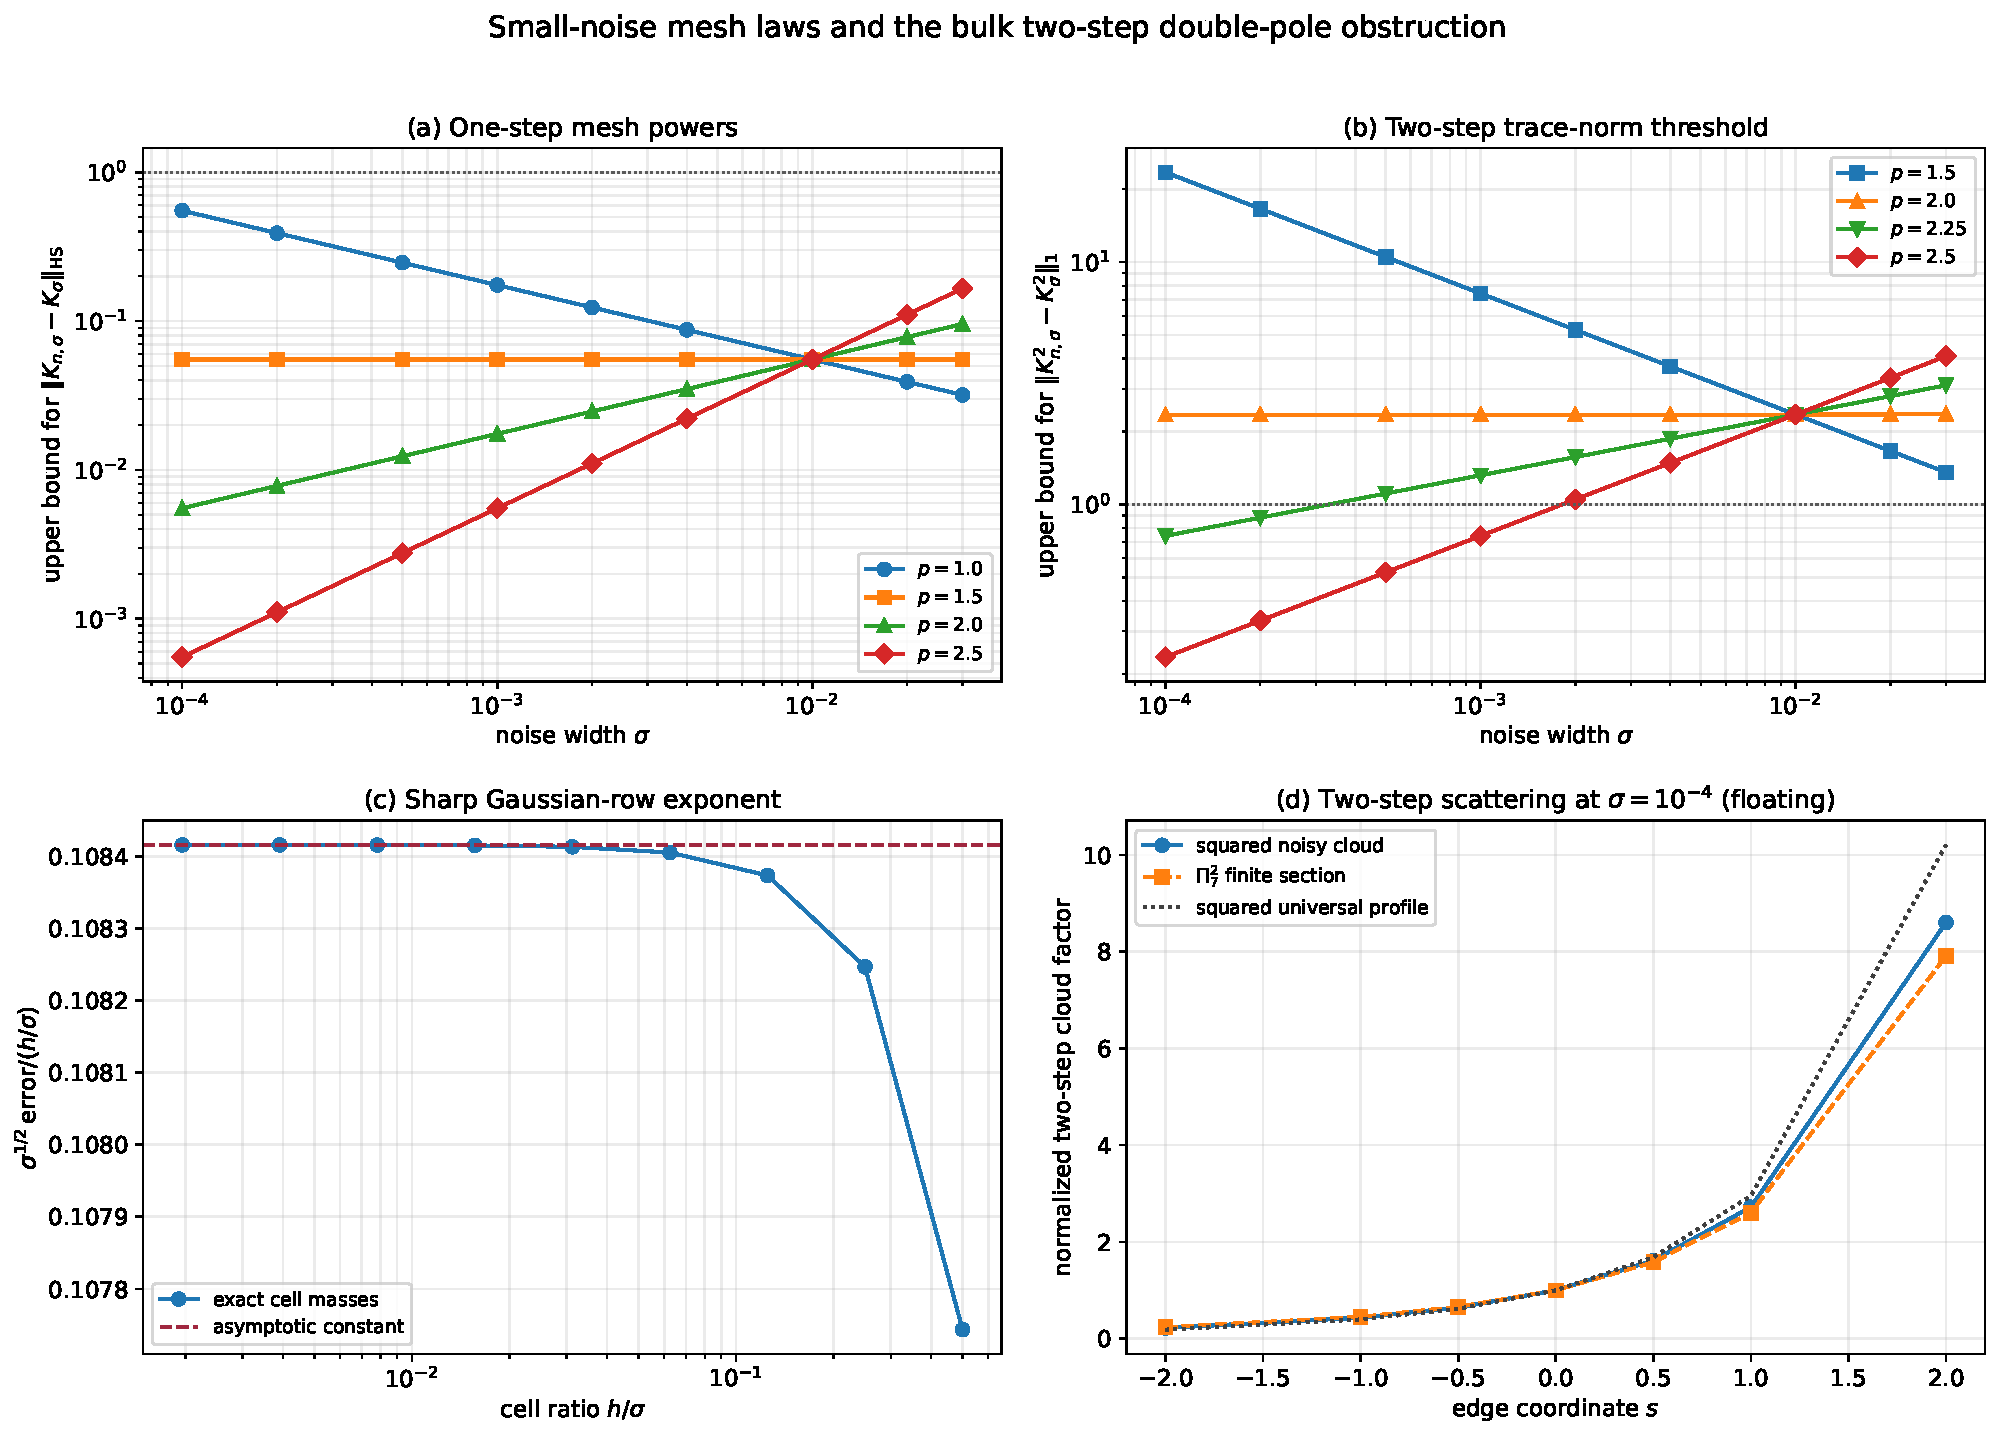
\includegraphics[width=\textwidth]{figures/small_noise_mesh_double_pole.pdf}
\caption{Small-noise mesh and pole-resolution summary.  (a) Explicit
Hilbert--Schmidt mesh bounds for $n_p(\sigma)\asymp\sigma^{-p}$; $p=3/2$
is critical.  (b) Bulk-free Markov square trace-norm bounds; $p=2$ is
critical and $p>2$ decays.  (c) Exact normalized Gaussian cell masses recover
the sharp constant in \eqref{eq:sharp-row-law}.  (d) The archived
$\sigma=10^{-4}$ resonance cloud after squaring, compared with the exact
$\Pi_7^2$ finite section and its universal large-$N$ profile.  Panel (d) is
floating evidence only.}
\label{fig:summary}
\end{figure}

\section{What is closed and what remains}
\label{sec:boundary}

The maze now has two separately marked walls.
\begin{enumerate}[leftmargin=2em]
 \item \textbf{Spatial wall.}  Absolute Hilbert--Schmidt approximation of a
 narrowing Gaussian kernel requires more than fixed points per noise width.
 The canonical sufficient scales are $n\sigma^{3/2}\to\infty$ at one step
 and $n\sigma^2\to\infty$ for trace-norm squares.
 \item \textbf{Analytic wall.}  Even perfect continuum resolution cannot
 yield an unrenormalized entire small-noise two-step determinant.  The
 coefficient germ has a genuine double pole at $w=\lambda$.
\end{enumerate}

The next positive gate is correspondingly precise: prove a moving-contour
weighted-Riesz theorem strong enough to determine the exponents $q,r$ in
\cref{cond:peripheral}.  A uniform resolvent bound would retain the
$p>2$ two-step mesh law.  Polynomial resolvent growth would quantify exactly
how much faster the grid must grow.

Beyond that contour gate, the determinant must be renormalized by an actual
noisy cloud factor.  The canonical candidate is
\begin{equation}
 \Pi_{N_\sigma}(w/\lambda)^2,
 \label{eq:renormalizer-candidate}
\end{equation}
with the rank clock \eqref{eq:rank-clock}.  Proving that division by the
actual cloud leaves a normal residual family would convert the negative
double-pole theorem into a positive scattering continuation.

None of these statements identifies a trace with primes or prime powers,
constructs a self-adjoint operator, derives a $T\log T$ counting law, or
locates a Riemann zero.  The result is a resolution and complex-analytic
theorem for one explicit noisy dynamical family.

\section*{Data and code availability}

All source code, certificates, floating pilots, tests, figures, hashes, and
the manuscript are available in
\url{https://github.com/maris205/prime_dynamics_theory/tree/main/papers/RH-46-small-noise-mesh-double-pole}.

\bibliographystyle{plainnat}
\bibliography{references}

\end{document}
